\chapter[Decaimiento del falso vacío en la TCC]{Decaimiento del falso vacío en la Teoría Cuántica de Campos}

%\section{Soluciones a la ecuación de movimiento}

\section{Tasa de decaimiento del falso vacío por unidad de volumen
	%en la Teoría Cuántica de Campos
}

Consideremos el campo escalar $\phi\qty(x)$ cuya acción $S\qty[\phi\qty(x)]$ está dada por %\footnote{$x=\qty(t, x, y, z)$ es el cuadrivector posición.} 
\begin{equation} \label{eq:accion_qft}
S\qty[\phi\qty(x)] = \int \dd[4]{x} \qty[\frac{1}{2}\qty(\pdv{\phi}{t})^2 - \frac{1}{2}\qty(\grad{\phi})^2 - U\qty(\phi) ]
\end{equation}
donde el potencial 
%\footnote{$U\qty(\phi)$ es la densidad de potencial pero por comodidad no usaremos esta denominación.} 
$U\qty(\phi)$ está dado en la figura \ref{fig:potencial_qft}. Cuenta con dos mínimos $\phi_-$ y $\phi_+$, de los cuales este último es un falso vacío por lo que, al igual que en la Mecánica Cuántica, 
%revisar terminos: "se encuentre" o "tenga una configuracion"
esperamos que, si la configuración inicial del campo es $\phi_+$, 
exista una cierta probabilidad de que
pueda decaer a $\phi_-$ por tunelamiento. Resulta conveniente añadirle una constante 
%a $U\qty(\phi)$ 
de tal manera que $U\qty(\phi_+) = 0$ y la energía del campo en el falso vacío sea finita \cite{andreassen2017precision}. 
\begin{figure}[t]
	\centering
	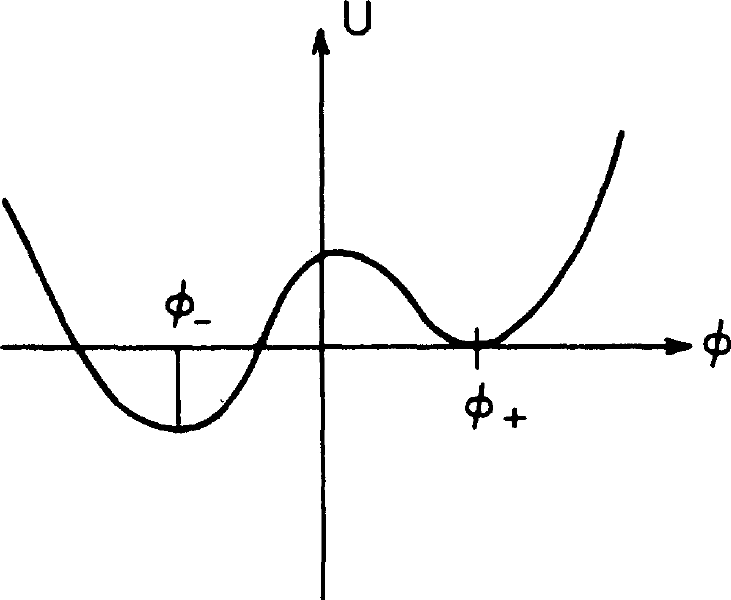
\includegraphics[scale=0.25]{FIGURAS/potencial_qft}
	\caption{Potencial en el que se encuentra el campo escalar dado por la acción \eqref{eq:accion_qft}. Notamos que cuenta con un falso vacío en $\phi_+$ \cite{callan1977fate}.}
	\label{fig:potencial_qft}
\end{figure}

A pesar de esto, la energía del campo en el verdadero vacío es infinita debido a que $U\qty(\phi_-)$ es distinto de cero e integramos sobre todo el espacio \cite{paranjape2017theory}. De la misma manera, la barrera de potencial a través de la cual se debe dar el tunelamiento, también es infinita, por lo que el decaimiento del falso vacío solo puede darse en ciertas regiones del espacio. 
%Como esta es arbitraria, la tasa de decaimiento es proporcional al volumen y por lo tanto, infinita \cite{weinberg2012classical}.  
%añadir algo sobre que la diferencia de energia respecto al falso vacio es finita
Es por esto que la cantidad físicamente relevante a calcular es la tasa de decaimiento del falso vacío por unidad de volumen $\Gamma/V$ \cite{weinberg2012classical} de la forma
\begin{equation} \label{eq:gamma_volumen_WKB}
\frac{\Gamma}{V} = Ae^{-B/\hbar}\qty(1 + \order{\hbar}),
\end{equation}
% serán discutidas más adelante. 
donde $A$ y $B$ son coeficientes a determinar mediante la extensión del formalismo desarrollado en el capítulo anterior a la Teoría Cuántica de Campos del campo escalar. 

\section{Bounces en la Teoría Cuántica de Campos}

%Habiendo desarrollado el formalismo 
Si bien al momento de calcular $\Gamma/V$ haremos uso del formalismo desarrollado en el capítulo anterior,
%adaptado, mediante analogía con lo estudiado 
previamente debemos plantear el problema clásico correspondiente con sus respectivas condiciones de frontera y encontrar 
%las configuraciones clásicas  
las configuraciones clásicas del campo que no son más que las soluciones a la ecuación de movimiento.  

Al aplicar el cambio de variable a tiempo imaginario \eqref{eq:tiempo_im} en la acción \eqref{eq:accion_qft} tenemos que $\phi = \phi\qty(\vb{x}, \tau)$ \footnote{A partir de ahora trabajaremos exclusivamente en tiempo euclideano. 
%en lo que resta de la sección 
%por lo que  omitiremos la dependencia funcional de $\phi = \phi\qty(\tau, \vb{x})$ en la medida de lo posible.
} 
y su acción euclideana $S_E\qty[\phi\qty(\tau, \vb{x})]$ está dada por
\begin{equation}
S_E\qty[\phi\qty(\vb{x}, \tau)] = \int \dd{\tau} \dd[3]{x} \qty[\frac{1}{2}\qty(\pdv{\phi}{\tau})^2 + \frac{1}{2}\qty(\grad{\phi})^2 + U\qty(\phi)]
\end{equation}
junto con la ecuación de movimiento correspondiente
\begin{equation} \label{eq:eom_phi}
\qty(\pdv[2]{\tau} + \grad{}^2)\phi = U'\qty(\phi),
\end{equation}
donde la prima indica la derivada respecto a $\phi\qty(\vb{x}, \tau)$. 

Como estamos interesados en las configuraciones clásicas,
%puesto que este es un punto estacionario de la acción. Inicialmente el campo se encuentra en el falso vacío
debemos establecer las condiciones de frontera adecuadas para la ecuación de movimiento \eqref{eq:eom_phi}. Sabemos que la solución no trivial relevante en el decaimiento del falso vacío es el bounce \cite{coleman1977fate}. Es decir, buscamos una configuración que parta de $\phi_+$, atraviese la barrera hasta llegar al punto de retorno y finalmente, regrese de vuelta a $\phi_+$.  De esta manera, podemos trasladar todas las consideraciones estudiadas anteriormente en la Mecánica Cuántica a la Teoría Cuántica de Campos del campo escalar. 

Tenemos entonces la primera condición de frontera 
%Bajo las mismas consideraciones 
\begin{equation} \label{eq:cond_frontera_qft1}
\lim_{\tau \rightarrow \pm\infty} \phi\qty(\vb{x}, \tau) = \phi_+,
\end{equation}
%donde hemos establecido $\tau_i = -\infty$ y $\tau_f = +\infty$ puesto que esperamos obtener el bounce en el límite . %puesto que este es el límite en el que estamos interesados. 
%que nos asegura que tanto la configuración inicial como final del campo es el falso vacío. 
la cual establece que el
%la configuración del 
campo permanece en el falso vacío durante un tiempo euclideano lo suficientemente largo antes y después de atravesar la barrera. Cabe resaltar que este comportamiento simétrico es debido al hecho de que la acción es invariante ante inversiones temporales. Como hemos establecido la condición de frontera \eqref{eq:cond_frontera_qft1} para un tiempo euclideano que tiende al infinito, 
%por conveniencia, 
podemos fijar el instante en el que el campo llega al punto de retorno en $\tau = 0$,
\begin{equation} \label{eq:cond_frontera_qft2}
\pdv{\phi}{\tau}\qty(\vb{x}, 0) = 0,
\end{equation}
%Podemos hacer esto debido al límite que estamos considerando.
%\begin{equation}
%	\mathcal{E} = \frac{1}{2}\qty(\pdv{\phi}{\tau})^2 - \frac{1}{2}\qty(\grad{\phi})^2 - U\qty(\phi)
%\end{equation}
de tal manera que la energía cinética del campo sea igual a cero una vez que haya cruzado la barrera. 
Por último, la acción del bounce debe ser finita. Caso contrario, el coeficiente $B$ en la ecuación \eqref{eq:gamma_volumen_WKB}, se anularía \cite{lee2005fate}. Como $U\qty(\phi_+) = 0$,
%\begin{equation}
%\mathcal{E} = \frac{1}{2}\qty(\pdv{\phi}{\tau})^2 - \frac{1}{2}\qty(\grad{\phi})^2 - U\qty(\phi)
%\end{equation}
\begin{equation} \label{eq:cond_frontera_qft3}
\lim_{\qty|\vb{x}| \rightarrow \pm\infty} \phi\qty(\vb{x}, \tau) = \phi_+,
\end{equation}
el campo se encuentra en el falso vacío a grandes distancias \cite{Masoumi:2015psa}. %\subsection{Soluciones a la ecuación de movimiento}
%Habiendo establecido las condiciones de frontera

\begin{figure}[t]
	\centering
	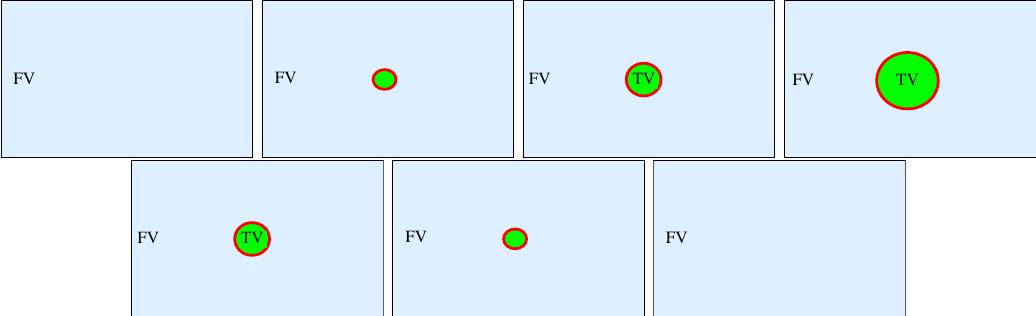
\includegraphics[scale=0.4]{FIGURAS/nucleacion_burbujas}
	\caption{Proceso de nucleación de una burbuja de verdadero vacío \cite{Masoumi:2015psa}.}
	\label{fig:nucleacionburbujas}
\end{figure}
Analicemos cualitativamente el comportamiento del bounce. Inicialmente, el campo se encuentra en el falso vacío a lo largo de todo el espacio.
%, tal como se indica en la primera condición de frontera \eqref{eq:cond_frontera_qft1}. 
En un cierto instante de tiempo euclideano y en una cierta región del espacio, el campo decae al verdadero vacío mientras que lejos de este, permanece inafectado. Es decir, aparece una burbuja de verdadero vacío 
%tal como se puede ver en la figura , %insertar figura
que empieza a crecer hasta alcanzar su tamaño máximo en $\tau = 0$, a partir del cual se encoge hasta desaparecer, regresando finalmente a la configuración inicial. Todo este proceso se ilustra en la figura \eqref{fig:nucleacionburbujas}
%Este proceso 
y es análogo al proceso de nucleación de burbujas de vapor en la Mecánica Estadística \cite{coleman1977fate}.
%, razón por la cual al bounce también se le denomina burbuja. 

Como es de esperarse, la ecuación de movimiento \eqref{eq:eom_phi} cuenta con una solución trivial que, de acuerdo con la condición de frontera en \eqref{eq:cond_frontera_qft1}, está dada por
\begin{equation} \label{eq:phi_trivial}
	\phi_{\text{FV}}\qty(\vb{x}, \tau) = \phi_+.
\end{equation}
%Tal como se expuso en el párrafo anterior, las soluciones no triviales 

Las ecuación de movimiento \eqref{eq:eom_phi}, las condiciones de frontera \eqref{eq:cond_frontera_qft1} y \eqref{eq:cond_frontera_qft3} y la interpretación del bounce como una burbuja de verdadero vacío, sugieren asumir que este último cuenta con una simetría $O\qty(4)$, es decir, es invariante ante rotaciones del espaciotiempo euclideano o esféricamente simétrico \cite{weinberg2012classical}. Para una gran cantidad de potenciales, esto siempre es posible 
%encontrar un bounce de esta forma 
\cite{coleman1978action}. 

Introduzcamos la distancia euclideana
\begin{equation}
	\rho^2 \equiv \vb{x}^2 + \tau^2
\end{equation}
de tal manera que, de acuerdo con lo establecido anteriormente,  $\phi = \phi\qty(\rho = \sqrt{\vb{x}^2 + \tau^2})$. 
%mientras que \eqref{eq:cond_frontera_qft2},
%\begin{equation}
%\eval{\pdv{\phi\qty(\rho)}{\tau}}_{\tau = 0} = 0.
%\end{equation}
%Como $\rho = \rho(\vb{x}, \tau)$, tenemos que
%\begin{equation}
%\pdv{\phi\qty(\rho)}{\tau} = \dv{\phi}{\rho}\pdv{\rho}{\tau}.
%\end{equation}
%
%\begin{align}
%	2\rho \pdv{\rho}{\tau} &= 2\tau \\
%	\pdv{\rho}{\tau} &= \frac{\tau}{\rho}
%\end{align}
%\begin{equation}
%\eval{\dv{\phi\qty(\rho)}{\tau}}_{\rho = 0} = 0
%\end{equation}
%\begin{equation}
%\eval{\dv{\phi}{\rho}}_{\rho = 0} = 0
%\end{equation}
Resulta conveniente renombrar las coordenadas espaciotemporales euclideanas como $\vb{x} = \qty(x_1, x_2, x_3)$ y $\tau = x_4$ de tal manera que podemos expresar $\rho$ y la ecuación de movimiento \eqref{eq:eom_phi} de forma compacta como
\begin{equation} \label{eq:rho_xi}
	\rho^2 = \sum_{i = 1}^{4} x_i^2
\end{equation}
%donde $\vb{x} = \qty(x, y, z) = \qty(x_1, x_2, x_3)$. 
%De acuerdo con esta notación, podemos escribir la ecuación de movimiento \eqref{eq:eom_phi} de forma comp
y 
\begin{equation} \label{eq:eom_xi}
\sum_{i = 1}^{4} \pdv[2]{\phi\qty(\rho)}{x_i} = U'\qty(\phi)
\end{equation}
respectivamente. 
Con esto, procederemos a desarrollar las derivadas 
%el cambio de variable 
en el lado izquierdo de la ecuación de movimiento \eqref{eq:eom_xi} para obtener  
%fácilmente 
la correspondiente a $\phi\qty(\rho)$. 
%nos facilitará el cambio de variable. 
%Empecemos por las primeras derivadas de $\phi\qty(\rho)$ respecto a $x_i$. 

Haciendo uso de la regla de la cadena, 
\begin{equation} \label{eq:dv_phi_rho}
	\pdv{\phi\qty(\rho)}{x_i} = \dv{\phi}{\rho}\pdv{\rho}{x_i}.
%	&= \frac{x_i}{\rho}\dv{\phi}{\rho},
\end{equation}
donde $i = 1, 2, 3, 4$. 
Derivemos la ecuación \eqref{eq:rho_xi} respecto a $x_i$ para obtener la derivada de $\rho$ respecto a $x_i$, 
%y simplificando,
\begin{align}
2\rho \pdv{\rho}{x_i} &= 2x_i \\ \label{eq:dv_rho_xi}
\pdv{\rho}{x_i} &= \frac{x_i}{\rho}.
\end{align}
%de tal manera que 
Al reemplazarla 
%esta última 
%\eqref{eq:dv_rho_xi} 
en la ecuación \eqref{eq:dv_phi_rho}, 
\begin{equation} \label{eq:dv_phi_rho2}
\pdv{\phi\qty(\rho)}{x_i} = \frac{x_i}{\rho}\dv{\phi}{\rho}.
\end{equation}
%\colorbox{yellow}{inicio revisar}
De igual manera, %calculemos las segundas derivadas de $\phi\qty(\rho)$ respecto a $x_i$ 
%derivando la ecuación \eqref{eq:dv_phi_rho2}
%respecto a $x_i$ y usando la ecuación \eqref{eq:dv_rho_xi},
\begin{align}
	\pdv[2]{\phi\qty(\rho)}{x_i} &= \frac{x_i}{\rho}\dv[2]{\phi}{\rho}\pdv{\rho}{x_i} + \qty(\frac{1}{\rho} - \frac{x_i}{\rho^2}\pdv{\rho}{x_i})\dv{\phi}{\rho} \\
	&= \frac{x_i^2}{\rho^2}\dv[2]{\phi}{\rho} + \frac{1}{\rho}\qty(1 - \frac{x_i^2}{\rho^2})\dv{\phi}{\rho}. 
\end{align}
Por último, al sumar las segundas derivadas
%\begin{align}
%\sum_{i = 1}^{4} \pdv[2]{\phi\qty(\rho)}{x_i} &=  \frac{\sum_{i = 1}^{4} x_i^2}{\rho^2}\dv[2]{\phi}{\rho} + \frac{1}{\rho}\qty(4 - \frac{\sum_{i = 1}^{4} x_i^2}{\rho^2})\dv{\phi}{\rho},
%\end{align}
%De la ecuación \eqref{eq:rho_xi}, las sumas en el lado derecho son iguales a $\rho^2$. 
y simplificar, obtenemos finalmente la ecuación de movimiento 
%en términos de $\phi\qty(\rho)$
\begin{equation} \label{eq:eom_rho}
	\dv[2]{\phi}{\rho} + \frac{3}{\rho}\dv{\phi}{\rho} = U'\qty(\phi).
\end{equation}

Las condiciones de frontera \eqref{eq:cond_frontera_qft1} y \eqref{eq:cond_frontera_qft3} se reducen a 
\begin{equation} \label{eq:cond_frontera_rho1}
\lim_{\rho \rightarrow \pm\infty} \phi\qty(\rho) = \phi_+.
\end{equation}
Con la finalidad de evitar que las soluciones cuenten con una singularidad en el origen, requerimos que \cite{coleman1977fate}
\begin{equation} \label{eq:cond_frontera_rho2}
	\eval{\dv{\phi}{\rho}}_0 = 0.
\end{equation}

Podemos interpretar la ecuación de movimiento \eqref{eq:eom_rho} como la de una partícula con ``posición'' $\phi$ y ``tiempo'' $\rho$ moviéndose en el potencial invertido $-U\qty(\phi)$ bajo la acción de una fuerza de fricción cuyo coeficiente de amortiguamiento \footnote{Coeficiente de Stokes.} es inversamente proporcional al ``tiempo'' \cite{weinberg2012classical}. 
%analisis clasico de la eom
Es posible demostrar la existencia de una solución a esta ecuación que satisfaga las condiciones de frontera \eqref{eq:cond_frontera_rho1} y \eqref{eq:cond_frontera_rho2} mediante un argumento \emph{overshoot-undershoot} y la continuidad de las condiciones iniciales  \cite{coleman1977fate}.
%\colorbox{yellow}{fin revisar}
%\subsection{Aproximación de la pared delgada}
%
%El campo dentro de la burbuja, en realidad corresponde al punto de retorno y no al verdadero vacío \colorbox{yellow}{añadir citacion tesis lee}. 

\section{Aproximación de la pared delgada}

Podemos continuar con el análisis del bounce bajo la suposición de que 
%la diferencia entre los mínimos del potencial 
\begin{equation}
	\epsilon \equiv U\qty(\phi_+) - U\qty(\phi_-)
\end{equation}
es pequeño en comparación con la altura de la barrera del potencial. A este régimen se le denomina como la aproximación de la pared delgada (\emph{thin-wall approximation}) debido a que, como veremos más adelante, la burbuja está separada del exterior, que aún se encuentra en el falso vacío, por una pared delgada. 

Consideremos el potencial
\begin{equation} \label{eq:potencial_tw}
U\qty(\phi) = U_0\qty(\phi) + \frac{\epsilon}{2a}\qty(\phi - a),
\end{equation} 
donde $U_0\qty(\phi)$ es un potencial simétrico
%\begin{equation}
%	U_0\qty(-\phi) = U_0\qty(\phi)
%\end{equation}
que cuenta con dos mínimos iguales en $\phi(\rho) = \pm a$ tal que
\begin{gather}
U_0\qty(-\phi) = U_0\qty(\phi) \\
U_0 \qty(\pm a) = 0 \\
U'_0 \qty(\pm a) = 0 \\
U''_0 \qty(\pm a) = \omega^2,
\end{gather}
%$U\qty(\phi)$ 
como se muestra en la figura \ref{fig:pareddelgada}. En este caso, $\phi_+ = -a$ y $\phi_- = a$. 
\begin{figure}[t]
	\centering
	\includegraphics[scale=0.45]{FIGURAS/pared_delgada}
	\caption{Potencial $U\qty(\phi)$ en la aproximación de la pared delgada \cite{paranjape2017theory}.}
	\label{fig:pareddelgada}
\end{figure}

Reemplazando \eqref{eq:potencial_tw} en la ecuación de movimento \eqref{eq:eom_rho},
\begin{equation} \label{eq:eom_rho_tw1}
\dv[2]{\phi}{\rho} + \frac{3}{\rho}\dv{\phi}{\rho} = U_0'\qty(\phi) + \frac{\epsilon}{2a}.
\end{equation}
Despreciamos el último término por ser de orden $\epsilon$. 

Analizando la ecuación \eqref{eq:eom_rho_tw1} en términos de una partícula moviéndose en el potencial invertido $-U_0'\qty(\phi)$, tenemos que, como la diferencia entre ambos mínimos es tan pequeña, s posible que una partícula que empieza su movimiento en $a$, no cuente con la suficiente ``energía'' para llegar a $-a$ debido a la fuerza de fricción  \cite{Masoumi:2015psa}. Es por esto que, antes de cruzar la barrera para llegar a $-a$, la partícula debe permanecer cerca a $a$ durante un tiempo $\rho \approx R$ lo suficientemente grande, de tal manera que el termino de fricción se vuelva despreciable \cite{weinberg2012classical}. 
La ecuación \eqref{eq:eom_rho_tw1} se reduce entonces,
\begin{equation} \label{eq:eom_rho_tw2}
\dv[2]{\phi}{\rho} = U_0'\qty(\phi).
\end{equation}

Notamos que la ecuación \eqref{eq:eom_rho_tw2} es de la misma forma que la ecuación de movimiento \eqref{eq:mov_ec}, por lo que podemos hacer uso del hecho de que 
%la energía euclideana correspondiente es igual a 0, es decir, 
\begin{equation}
\qty(\dv{\phi}{\rho})^2 - U_0\qty(\phi) = 0
\end{equation} 
para obtener la solución 
%que cumpla con las condiciones de frontera. 
%Despejando e integrando obtenemos
\begin{equation}
\rho - R = \int_0^{\phi_I \qty(\rho)} \frac{\dd{\phi}}{\sqrt{U_0\qty(\phi)}}
\end{equation}
conocida como instanton. A diferencia del bounce, 
%que también es una solución de esta ecuación 
 el campo se encuentra en el verdadero vacío cerca al origen. 
%Para solucionar la ecuación hacemos uso del hecho de que la energía euclideana es igual a 0, es decir, 
%\begin{equation}
%\qty(\dv{\phi}{\rho})^2 - U_0\qty(\phi) = 0.
%\end{equation}
%Despejando e integrando obtenemos la solución
%\begin{equation}
%\rho - R = \int_0^{\phi_{\text{TW}}} \frac{\dd{\phi}}{\sqrt{U_0\qty(\phi)}}.
%\end{equation}
Tenemos entonces que, de acuerdo con las condiciones de frontera y la discusión realizada anteriormente, 
%sabemos que cerca al origen,
%cerca al origen 
%$\phi = \phi_{\text{TV}}$ mientras que para $r >> R$,
%lejos de este 
%$\phi = \phi_{\text{TV}}$. Juntando todo esto 
el bounce en la aproximación de la pared delgada está dado por
\begin{equation} \label{eq:bounce_tw}
\phi_B \qty(\rho) = \begin{cases}
%\phi_{\text{TV}} =
-a & 0 < \rho \ll R \\
\phi_I \qty(\rho) & \rho \approx R \\
%\phi_{\text{FV}}  =
a & \rho \gg R
\end{cases}.
\end{equation}
donde $R$ es el radio de la burbuja. 

Como ejemplo explícito consideremos
\begin{equation}
U_0\qty(\phi) = \frac{\lambda}{8}\qty(\phi^2 - a^2),
\end{equation}
de tal manera que la solución a la ecuación \eqref{eq:eom_rho_tw2} está dada por
\begin{equation}
\phi_{\text{TW}}\qty(\rho) = a\tanh(\frac{\omega}{2}\qty(\rho - R))
\end{equation}
donde $\omega^2 = \lambda^2 a^2$ \cite{das2006field}. En la figura, podemos apreciar que $\phi_{\text{TW}}\qty(\rho)$ presenta el comportamiento esperado, es decir, el campo se encuentra en el verdadero vacío cerca al origen hasta llegar a $\rho \approx R$ donde ocurre la transición al falso vacío. Esta región es una pared delgada que separa a la burbuja del exterior. 
\begin{figure}[t]
	\centering
	\includegraphics[scale=0.3]{FIGURAS/rho_tw}
	\caption{Bounce en la aproximación de la pared delgada. En la figura $r = \rho$, $\phi_+ = -\varphi_0$ y $\phi_- = \varphi_0$ \cite{rubakov2009classical}}
	\label{fig:rhotw}
\end{figure}

La acción euclideana del bounce %en coordenadas esféricas en $O\qty(4)$ %$B = S_E\qty[\phi_B\qty(\rho)]$
está dada por \cite{rubakov2009classical}
\begin{equation}
S_E\qty[\phi_B\qty(\rho)] = 2\pi^2 \int_0^{+\infty} \dd{\rho}  \rho^3 \qty[\frac{1}{2}\qty(\pdv{\phi_B}{\rho})^2 + U\qty(\phi_B)].
\end{equation}
En la aproximación de la pared delgada,
%el bounce es de la forma dada en la ecuación \eqref{eq:bounce_tw} por lo que debemos calcular la integral en cada 
\begin{align}
S_E\qty[\phi_B\qty(\rho)] &= 2\pi^2  \left( \int_0^{R - \Delta R/2} \dd{\rho}  \rho^3 U\qty(-a) +  \int_{R - \Delta R/2}^{R+\Delta R/2} \dd{\rho}  \rho^3 \qty[\frac{1}{2}\qty(\pdv{\phi_I}{\rho})^2 + U\qty(\phi_I)] \right. \\
&\phantom{= 2\pi^2 \left( \right. } \quad  \left. + \int_{R+\Delta R/2}^{+\infty} \dd{\rho}  \rho^3 U\qty(a) \right)
\end{align}
donde $\Delta R$ es el ancho de la pared tal que $R \gg \Delta R$. 
%Cada integral representa la contribución de cada región del 

Calculamos cada integral por separado. Como $U\qty(-a) = -\epsilon$, %la contribución del interior de la burbuja está dada por 
\begin{equation}
 \int_0^{R - \Delta R/2} \dd{\rho}  \rho^3 U\qty(-a) 
%-\frac{\epsilon}{2} \int_0^{R - \Delta\rho} \dd{\rho} \rho^3 \\
%-\epsilon \qty[\frac{\rho^4}{4}]_0^{R - \Delta R} \\
\approx -\frac{1}{4} R^4 \epsilon, %+ \order{\Delta\rho},
\end{equation}
donde ignoramos los términos del orden $\Delta R$, mientras que la última integral se anula debido a que $ U\qty(a) = 0$. En la segunda integral, $\rho \approx R$ por lo que
%se mantiene prácticamente constante cerca a la barrera, por lo que podemos considerarla igual a $R$ y sacarla de la integral %De la figura \ref{fig:rhotw}
\begin{equation}
\int_{R - \Delta R/2}^{R+\Delta R/2} \dd{\rho}  \rho^3 \qty[\frac{1}{2}\qty(\pdv{\phi_I}{\rho})^2 + U\qty(\phi_I)] \approx R^3 \int_{R - \Delta R/2}^{R+\Delta R/2} \dd{\rho} \qty[\frac{1}{2}\qty(\pdv{\phi_I}{\rho})^2 + U\qty(\phi_I)] 
\end{equation}
La integral del potencial $U\qty(\phi_I)$ se reduce a  %$\epsilon\qty(\phi - a)/2a$ se anula debido a que $\phi_{\text{TW}}\qty(\rho)$ es antisimétrica como se puede
\begin{align}
\int_{R - \Delta R/2}^{R+\Delta R/2} \dd{\rho}  U\qty(\phi_I) &= \int_{R - \Delta R/2}^{R+\Delta R/2} \dd{\rho} U_0\qty(\phi) + \frac{\epsilon}{2a}\qty(\int_{R - \Delta R/2}^{R+\Delta R/2} \dd{\rho}\phi\qty(\rho) - \int_{R - \Delta R/2}^{R+\Delta R/2} \dd{\rho}) \\ 
%&= \int_{R - \Delta R/2}^{R+\Delta R/2} \dd{\rho} U_0\qty(\phi) + \frac{1}{2}\epsilon\Delta R \\
&\approx \int_{R - \Delta R/2}^{R+\Delta R/2} \dd{\rho} U_0\qty(\phi)
\end{align}
donde la segunda integral se anula debido a que $\phi_I\qty(\rho)$ es antisimétrica, como se puede apreciar en la figura \ref{fig:rhotw}, mientras que la última se desprecia por ser del orden $\epsilon\Delta R$.

Tomando en cuenta todo lo anterior tenemos que la acción euclideana en la aproximación de la pared delgada está dada por
\begin{equation}
	S_E\qty(R) \approx -\frac{1}{2}\pi^2 R^4 \epsilon + 2\pi^2 R^3 S_I
\end{equation}
donde 
\begin{equation}
	S_I \equiv \int_{R - \Delta R/2}^{R+\Delta R/2} \dd{\rho}  \rho^3 \qty[\frac{1}{2}\qty(\pdv{\phi_I}{\rho})^2 + U_0\qty(\phi_I)].
\end{equation}
Como $S_E\qty(R)$ debe ser estacionario,
\begin{equation}
	\dv{S_E}{R} = -2\pi^2 R^2 \epsilon + 6\pi^2 R^3 S_I = 0
\end{equation}
de donde obtenemos que
\begin{equation}
	R = \frac{3S_I}{\epsilon}
\end{equation}
por lo que finalmente
\begin{equation}
	B = S_E\qty[\phi_B\qty(\rho)] = \frac{27}{2}\frac{\pi^2 S_I^4}{\epsilon^3}.
\end{equation}

\section{Cálculo de la tasa de decaimiento del falso vacío por unidad de volumen}

Habiendo obtenido las configuraciones clásicas relevantes en el decaimiento del falso vacío, procedemos al cálculo de la tasa de decaimiento del falso vacío por unidad de volumen $\Gamma/V$. Siguiendo el formalismo de Coleman y Callan, partimos de la amplitud de transición 
\begin{equation}
I = \bra{\phi_f}e^{-HT/\hbar}\ket{\phi_i} = \int \mathcal{D}\phi \, e^{-S_E\qty[\phi\qty(\vb{x},\tau)]/\hbar},
\end{equation}
donde $\phi_i$ y $\phi_f$ son las configuraciones inicial y final del campo respectivamente y $T$ es el intervalo de tiempo euclideano. A partir de este obtendremos $\Gamma/V$ que, de acuerdo con la ecuación \eqref{eq:Gamma}, está relacionado con la amplitud de transición como
%de la siguiente manera
\begin{equation} \label{eq:Gamma/V_amplitud}
\frac{\Gamma}{V} = 2\Im\qty(\lim_{T \rightarrow \infty} \frac{ \ln I}{T}).
\end{equation}
De acuerdo con la condición de frontera \eqref{eq:cond_frontera_qft1}, $\phi_i = \phi_f = \phi_+$. 

En la aproximación del punto estacionario, la amplitud de transición a primer orden en $\hbar$ está dada por
\begin{equation} \label{eq:I_phi}
I = e^{-S_E^{\textrm{cl}} / \hbar} \qty[ \det\left(-\pdv[2]{\tau} -\grad{} + U''\qty(\phi_{\textrm{cl}}) \right) ]^{-1/2} \qty(1 + \order{\hbar}).,
\end{equation}
donde $\phi_{\textrm{cl}}$ es la configuración clásica del campo correspondiente al punto estacionario de la acción euclideana y $S_E^{\textrm{cl}} = S[\phi_{\textrm{cl}}\qty(\vb{x}, \tau)]$ es su acción euclideana. En caso cuente con múltiples puntos estacionarios, debemos sumar la contribución de cada uno. 

Tal como vimos en el capítulo 
%\ref{cap:falso_vacio_qm}
anterior, las configuraciones clásicas a considerar son la trivial, el bounce o burbuja así como las configuraciones que cuenten con múltiples bounces. Nuevamente volveremos a encontrarnos con los mismo problemas al momento de calcular la contribución del bounce a la amplitud de transición, los cuales tendrán que ser tratadas independientemente. 

De acuerdo con la ecuación \eqref{eq:I_phi}, la contribución de la configuración trivial $\phi_{\text{FV}}\qty(\vb{x}, \tau)$ a la amplitud de transición $I_0$ no es más que
\begin{equation}
	I_0 = \qty[ \det\qty(-\pdv[2]{\tau} -\grad{} + \omega^2) ]^{-1/2},
\end{equation}
donde $\omega^2 \equiv U''\qty(\phi_+)$. De igual manera, esperaríamos que la contribución del bounce $\phi_B\qty(\vb{x}, \tau)$ a la amplitud de transición $I_1$ este dada por 
\begin{equation}
I_1 = e^{-B / \hbar} \qty[ \det\qty(-\pdv[2]{\tau} -\grad{} + U''\qty(\phi_B) ) ]^{-1/2},
\end{equation}
donde $B = S[\phi_B\qty(\vb{x}, \tau)]$ es la acción euclideana del bounce. Sin embargo, sabemos que esta expresión no es la correcta puesto que no todos los autovalores del operador
\begin{equation}
	\hat{O} \equiv -\pdv[2]{\tau} -\grad{} + U''\qty(\phi_B)
\end{equation}
son positivos. 

Las burbujas pueden aparecer en cualquier región del espacio, es decir, son invariantes ante traslaciones espaciales \cite{coleman1977fate}. Además, aunque fijamos el instante en el que el campo llega al punto de retorno en $\tau = 0$, bien podríamos haberlo hecho en cualquier otro instante de tiempo euclideano. Ambas observaciones indican que el bounce es invariante ante traslaciones espaciotemporales en el espaciotiempo euclideano. Esto significa que, al igual que lo que ocurría con el bounce en la Mecánica Cuántica, el operador $\hat{O}$ cuenta con modos ceros 
%por lo que su determinante no está bien definida. 
Nuevamente, esto es un reflejo de la simetría $O(4)$ del sistema. 
En esta ocasión, tendremos cuatro modos ceros
\begin{equation}
	\phi_{0_i}\qty(\vb{x}, \tau) = \qty(\frac{B}{2\pi\hbar})^{-1/2}\pdv{\phi_B}{x_i},
\end{equation}
donde $i = 1, 2, 3, 4$. Al 
%hacer el cambio de variable de los coeficientes respectivos 
integrar sobre el centro de la burbuja 
%a lo largo de una cierta región d
en el espaciotiempo euclideano, 
%la contribución del bounce a la amplitud de transición 
$I_1$ adquiere el siguiente factor
\begin{equation}
	\qty(\frac{B}{2\pi\hbar})^{2}VT.
\end{equation}
%debido  factor de $\qty(B/2\pi\hbar)^{-1/2}$ por cada uno de estos, además de $TV$ debido al volumen del espaciotiempo euclideano sobre el cual hemos integrado.  

Es posible demostrar que el operador $\hat{O}$ cuenta con único modo negativo %en todos los casos de interés 
\cite{coleman1977fate, coleman1988quantum}. Para solucionar este problema, hacemos la continuación analítica de la integral de camino euclideana \eqref{eq:I_phi} deformando el contorno de integración a la parte superior del plano complejo. Como resultado, $I_1$ obtiene un factor de adicional de $i/2$, por lo que la contribución del bounce a la amplitud de transición es en realidad 
\begin{equation}
I_1 = e^{-B / \hbar} \qty(\frac{B}{2\pi\hbar})^{2}VT \qty[ \textrm{det}'\left(-\pdv[2]{\tau} -\grad{} + U''\qty(\phi_B) \right) ]^{-1/2},
\end{equation}
donde la prima en la determinante indica que se ha excluido el autovalor igual a cero. 

Por último, consideremos las configuraciones que cuentan con un número arbitrario de $n$ bounces lo suficientemente separados. Siguiendo el análisis realizado en el capítulo anterior, sabemos que, al sumar todas las contribuciones de estas configuraciones, la amplitud de transición \eqref{eq:I_phi} está dada por
\begin{equation} \label{eq:I_phi_final}
	I = I_0 \exp\qty(iKVTe^{-B/\hbar}),
\end{equation}
donde
\begin{equation}
K \equiv \frac{1}{2} \left(\frac{B}{2\pi\hbar}\right)^2 \qty[ \frac{\textrm{det}' \qty(-\pdv[2]{\tau} -\grad{} + U''\qty(\phi_B) )}{\det \qty(-\pdv[2]{\tau} -\grad{} + \omega^2 )} ]^{-1/2}.
\end{equation}

Finalmente, reemplazando la amplitud de transición \eqref{eq:I_phi_final} en la ecuación \eqref{eq:Gamma/V_amplitud}, obtenemos la tasa de decaimiento del falso vacío por unidad de volumen $\Gamma/V$ a primer orden en $\hbar$
\begin{equation} \label{eq:gamma_final_V}
\frac{\Gamma}{V} = \qty(\frac{B}{2\pi\hbar})^2  \qty[ \frac{\textrm{det}' \qty(-\pdv[2]{\tau} -\grad{} + U''\qty(\phi_B) )}{\det \qty(-\pdv[2]{\tau} -\grad{} + \omega^2 )} ]^{-1/2}e^{-B/\hbar}\left( 1 + \mathcal{O}(\hbar)\right).
\end{equation}

\section{El destino del falso vacío}

%\subsection{Evolución de las burbujas de verdadero vacío}

%Habiendo obtenido la tasa de decaimiento del falso vacío por unidad de volumen, 
Analicemos la evolución de una burbuja de verdadero vacío en el espaciotiempo de Minkowski. Al cruzar la barrera de potencial a través de un salto cuántico en $t = 0$, el campo emerge en el punto de retorno en la configuración más probable, es decir, 
\begin{equation}
	\phi\qty(\vb{x}, t = 0) =  \phi_B\qty(\vb{x}, \tau = 0),
\end{equation}
debido a que el bounce es la configuración que cuenta con la menor acción euclideana \cite{rubakov2009classical}. Además, 
\begin{equation} 
\pdv{\phi}{t}\qty(\vb{x}, t = 0) = 0,
\end{equation}
y a partir de este instante, el campo evoluciona de acuerdo con la ecuación de movimiento \cite{callan1977fate}
\begin{equation} \label{eq:eom_minkowski}
	\qty(\pdv[2]{\tau} - \grad{}^2)\phi\qty(\vb{x}, t) = -U'\qty(\phi\qty(\vb{x}, t)).
\end{equation}
Tenemos entonces que en $t = 0$, se materializa una burbuja de verdadero vacío de radio $R$. 
%Es decir, en $t = 0$, se materializa. 

\begin{figure}[t]
	\centering
	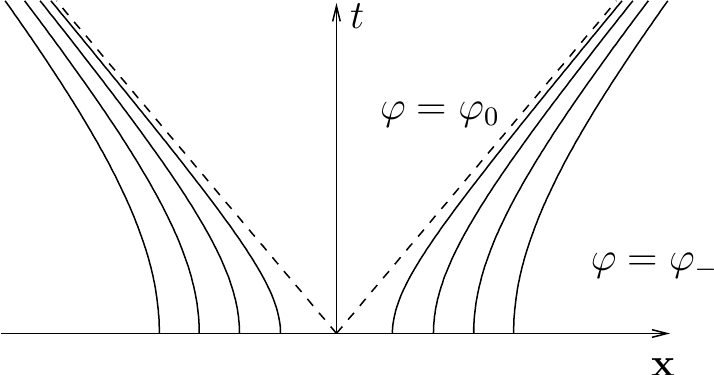
\includegraphics[scale=0.35]{FIGURAS/bubble_growth}
	\caption{Crecimiento de las burbujas de verdadero vacío en el espaciotiempo de Minkowki. En la figura, $\varphi_-$ y $\varphi_0$ corresponden al falso y verdadero vacío respectivamente \cite{rubakov2009classical}.}
	\label{fig:bubblegrowth}
\end{figure}

Para obtener $\phi\qty(\vb{x}, t)$ hacemos el cambio de variable $ \tau = it$ en la ecuación \eqref{eq:rho_xi} para pasar del tiempo euclideano al del espaciotiempo de Minkowski. Definamos
\begin{equation}
	r^2 \equiv \vb{x}^2 - t^2,
\end{equation}
de tal manera que al hacer la continuación analítica del bounce al campo en el espaciotiempo de Minkowski tenemos que este último está dado por
\begin{equation} 
	\phi\qty(\vb{x}, t) = \phi_B\qty(r = \sqrt{\vb{x}^2 - t^2}) 
	%= \phi_B\qty(\rho = \sqrt{\vb{x}^2 + \tau^2}).
\end{equation}
Puesto que $r$ es positivo, esta solución solo está definida fuera del cono de luz. Para obtener la solución dentro del cono de luz habría que resolver la ecuación de movimiento \eqref{eq:eom_minkowski} \cite{weinberg2012classical}. 
La simetría $O(4)$ del bounce se ha convertido entonces en una simetría $O(3, 1)$. Esto significa que la evolución de la burbuja será la misma para cualquier observador inercial \cite{coleman1977fate}. A medida que la burbuja se expande, su pared describe la hiperboloide
\begin{equation}
\vb{x}^2 - t^2 = R^2
\end{equation}
tal como se puede apreciar en la figura \eqref{fig:bubblegrowth}. Es decir, la burbuja crece a una velocidad que se aproxima a la velocidad de la luz asintóticamente. Si $R$ es microscópico, del orden de $10^{-10}$, esto es prácticamente instantáneo  de tal manera que si una burbuja se está acercando, no sabremos en qué momento nos golpeó \cite{paranjape2017theory}. Dentro de la burbuja solo queda el verdadero vacío inalterado.

%\subsection{Implicaciones cosmológicas}

%\subsection{Aplicaciones}